
\subsubsection*{Problem definition}

This diffusion model is built to reproduce a field study in clay. This in situ test consists of a borehole where a solution is circulated that contains tracer substances like HTO. These tracers diffuse into the adjacent clay. The aim of the investigation is to simulate the HTO distribution after 300 d, the final test time, and to compare the simulation results of GeoSys/RockFlow to those that are calculated by HYDRUS 1~D (Simunek et al.) and PHAST (Parkhurst et al.).

\subsubsection*{Model set-up of the 1~D axisymmetric model}

To build a proper model of the tracer test, a one-dimensional axisymmetric model with 3.8~cm of borehole radius and 21.2~cm horizontal distance in the clay soil is created. As initial condition a constant pressure of 0 was specified in the whole model and the concentration relation c/c$_0$ of 1 within the distance of the borehole radius and of 0 within the clay domain. The pressure boundary condition corresponds to the initial condition. The calculation model includes 310 elements and 311 nodes. Table \ref{tab53} shows the used parameters for the clay and the apparent diffusion constant D$_a$ of HTO. The calculation is performed for the test duration of 300 days with fitted time step lengths from 0.001~d to 1~d (Bahr, 2007). The porosity in the modelled borehole is assumed to be 1 in order to evoke the simulation of a tracer reservoir that supplies the tracer solution into the clay.

\begin{table}[htbp]
\centering
\begin{tabular}{|l|l|l|}
\hline
parameter & value & unit \\
\hline
density $\rho$  & 2.5 & t $\cdot$ m$^{-3}$  \\			
\hline
porosity $\Phi$ & 0.15 & -- \\
\hline
permeability $K$ & 1.0$\cdot 10^{-11}$ & m$^2$ \\
\hline
diffusion coefficient D$_a$ & 3.6$\cdot 10^{-10}$ & m$^2\cdot s^{-1}$  \\
\hline
\end{tabular}
\caption{Parameters}
\label{tab53}
\end{table}

\subsubsection*{Evaluation method}
The aim of the presented calculation example is the evaluation of the GeoSys/RockFlow-simulation results by comparing them with numerical results of two other simulation programmes. The comparison is made by the use of Hydrus 1~D, which is a one-dimensional transport model especially for the solute transport in soils. The second programme, PHAST, is linked to the chemical software PHREEQC. The simulation with both programmes was made under consideration of the same boundary conditions and parameters (Bahr, 2007).

\begin{figure}[htbp]
\centering
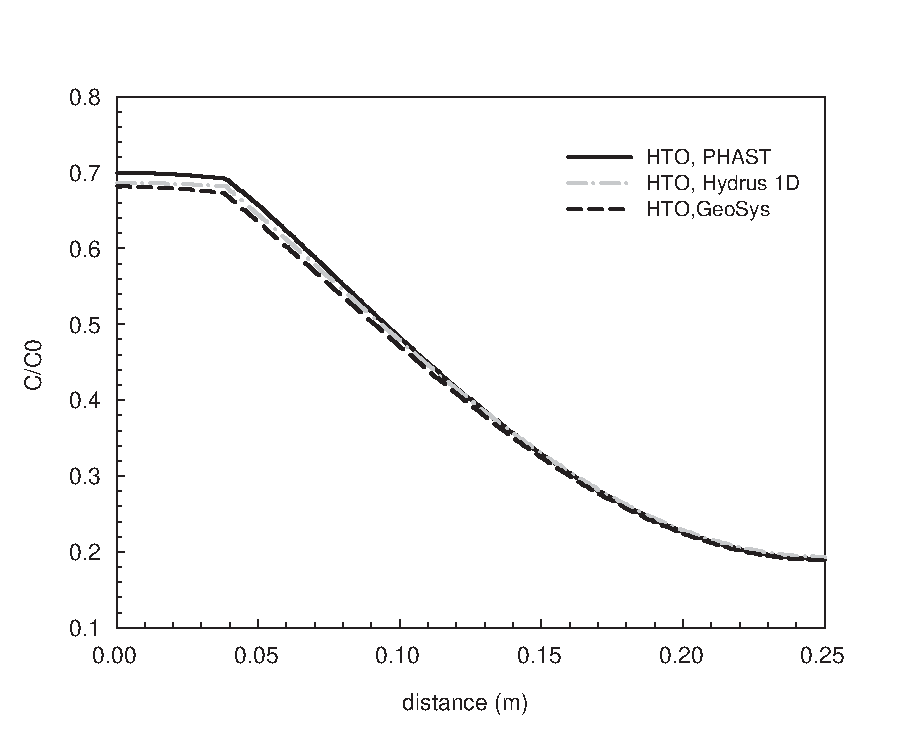
\includegraphics[width=0.8\textwidth]{C/figures/fig510.EPS}
\caption{Concentration distributions after 300~d}
\label{fig510}
\end{figure}

\subsubsection*{Results}

In figure \ref{fig510} you can find the concentration distributions over the width of 0.25~m after a simulation time of 300 days that were calculated by means of GeoSys/RockFlow, PHAST and Hydrus 1D (Bahr, 2007). The numerical results accord well to each other. Thus, the comparison shows that the diffusion process can be well reproduced by the use of an axisymmetric GeoSys/RockFlow model.

\begin{tabular}{|l|l|l|}
\hline
Benchmark & Problem type	& Path in benchmark deposit \\
\hline	
Diff\_HTO\_test	& HC	& benchmarks $\backslash$HC$\backslash$Diffusion$\backslash$ \\
\hline	
\end{tabular}
